


\documentclass[a4paper,10pt]{article}
%\documentclass[a4paper,10pt]{scrartcl}
\usepackage{hyperref}
\usepackage[utf8]{inputenc}
\usepackage[brazil]{babel}
\usepackage[T1]{fontenc}

\usepackage{graphicx}
\usepackage{amsmath}
\usepackage{indentfirst}
\usepackage{fancyhdr}
\usepackage{subfig}
\usepackage{setspace}
\usepackage{geometry}
\newcommand{\HRule}{\rule{\linewidth}{0.5mm}}
\usepackage{xcolor}
\usepackage{cite}  % Needed to use citations.  
\definecolor{verde}{rgb}{0.25,0.5,0.35}
\definecolor{jpurple}{rgb}{0.5,0,0.35}
\usepackage{listings}
\usepackage{float}

\lstset{
  language=Java,
  basicstyle=\ttfamily\small,
  keywordstyle=\color{jpurple}\bfseries,
  stringstyle=\color{red},
  commentstyle=\color{verde},
  morecomment=[s][\color{blue}]{/**}{*/},
  extendedchars=true,
  showspaces=false,
  showstringspaces=false,
  numbers=left,
  numberstyle=\tiny,
  breaklines=true,
  backgroundcolor=\color{cyan!10},
  breakautoindent=true,
  captionpos=b,
  xleftmargin=0pt,
  tabsize=4
}
\pagestyle{empty}
% Formatação
\topmargin -1.5cm
\oddsidemargin -0.04cm
\evensidemargin -0.04cm
\textwidth 16.59cm
\textheight 21.94cm 


\pdfinfo{%
  /Title    ()
  /Author   ()
  /Creator  ()
  /Producer ()
  /Subject  ()
  /Keywords ()
}

\begin{document}

\begin{titlepage}

\begin{center}

\includegraphics[width=0.15\textwidth]{./imgs/IME.png}\\[1cm]
\textsc{\Large Instituto de Matemática e Estatística\\ Universidade de São Paulo}\\[0.5cm]
{\large Bacharelado em Ciências da Computação}\\[5.0cm]
\HRule \\[0.4cm]
{\huge \bfseries Library Mapper} 
\HRule \\[1.0cm]

\begin{flushleft} \large
{\large Thiago Gomes Toledo\\ Supervisor: Prof. Dr. Marcelo Finger}
\end{flushleft}
\vfill

{\large São Paulo - SP\\[0.5cm] Segundo semestre de 2011}
\end{center}
\end{titlepage}

\newpage

\textit{ Agradeço a minha mãe Mara Lucia Gomes Toledo e a meu pai João Batista Toledo por terem me dado a oportunidade de realizar 
meu sonho; A OPUS-Software por proporcionar diversos recursos para a realização desse sonho; A minha esposa Lucianna Thomaz Almeida Toledo por me dar conforto, ajuda e sábias dicas; A meu filho que me traz
alegria só por imaginar seu rosto e a Deus por ter me dado todos e tudo que sempre precisei.}


\footnote[1]{Para mais informações sobre essa monografia, apresentação, código, etc.. acesse o site: \href{''http://www.linux.ime.usp.br/~renoir/mac499/proposta.html''}{www.linux.ime.usp.br/~renoir/mac499/proposta.html}}
\newpage
 \tableofcontents
\newpage
    \section{Introdução}
   
    Como frequentador da biblioteca do Instituto de Matemática e 
    Estatística da USP desde 2008 e trabalhando na biblioteca do Instituto de Geociencias da USP em 2010-2012, 
    pude notar que as reclamações numa biblioteca sobre a dificuldade em se achar um livro lideram o ranking de 
    problemas apontados por visitantes que usualmente têm que apelar para a boa vontade dos funcionários, 
    pois acham muito complicado ou até sem nenhum sentido o modo como as fileiras de livros são identificadas.\\
    
    Em ambos os casos os alunos ainda eram capazes de encontrar seus livros ou teses dado que a maior delas possuia
    não mais que 20.000 exemplares.Contudo, numa biblioteca como a da Faculdade de Filosofia, Letras e Ciências Humanas
    que hoje possui um inventório de mais de 500 mil livros e ainda 600 mil teses\footnote[1]{Dados levantados em janeiro 2012 com a diretora da biblioteca, Maria Aparecida Laet}, a busca se torna completamente inviável
    sem nenhum auxílio real.\\
   
    
    \section{Parte Objetiva}
    Nessa parte do texto, serão apresentados os conceitos teóricos do trabalho, além da parte prática
    de desenvolvimento.

    \subsection{Objetivo}
    Com uma ferramenta que mostre como ir do ponto onde está o visitante até o livro através de um mapa, esse dificilmente se sentiria perdido 
    ou precisaria contar com o auxílio de terceiros.Portanto, o objetivo desse projeto Library Mapper é que o vistante
    busque, escolha o livro e receba no seu aparelho mobile um mapa com o caminho correto até esse livro.
    
    \subsection{Problema}

    Como dispositivos GPS não mapeam dentro de residências, é inviável utilizar a Geolocalização do visitante para qualquer fim e portanto
    era necessário criar algum método para identificar onde ele estava localizado, como era esse lugar e como gerar uma busca
    entre onde ele estava e onde devia chegar.
    
    
    \subsection{Solução}
    
  Inicialmente desenvolvida para dispositivos IOS, essa ferramenta utiliza tags com códigos QR para auxiliar 
  o reconhecimento da localização atual do visitante.\\

  O visitante ao entrar numa biblioteca procura essa tag e com seu dispositivo IOS, reconhece o código 
  nela contido.Esse código abre um Web Browser no dispositivo e uma página da biblioteca na internet é 
  mostrada na tela.O visitante digita o livro num campo de busca e uma vez que esse existe nessa biblioteca, 
  a tela do web browser é substituída por uma tela com um mapa que mostra o caminho da tag selecionada 
  até a fileira onde esta o livro.\\
  
   Para ser possível a localização do livro, será utilizada a prévia catalogação feita pela biblioteca da 
   posição do mesmo e uma réplica proporcional do mapa real da biblioteca .Essa réplica
   é desenvolvida através de uma plataforma web que gera mapas 2D também desenvolvida nesse projeto.As informações
   obtidas nesse mapa, localização de estantes e suas correspondentes identificações, Qr-Codes, obstáculos e limites
   da biblioteca, serão enviados e armazenados num banco de dados da aplicação.\\
   
   
   
   
   O mapa será gerado num grafo tipo grid e cada nó está dividido em 4 tipos principais que são QR-Code, Forbidden, Free e Bookshelf 
   numa classe Node e será baseado nesses tipos que a busca pelo livro dado será feita.\\

   Como todas as arestas destre grafo tem peso único um, o algoritmo de busca usado é uma Bi-direcional BFS (Breadth-first search) com uma busca saindo da origem(QR-Code
   selecionado pelo visitante) e outra do destino (estante onde está o livro).\\

Essa busca é feita de uma maneira paralela onde cada thread é um dos pólos do caminho Bi-direcional.\\ 
  
    \subsection{Conceitos e tecnologias estudadas}
	\begin{figure}[H]
	\centering
      	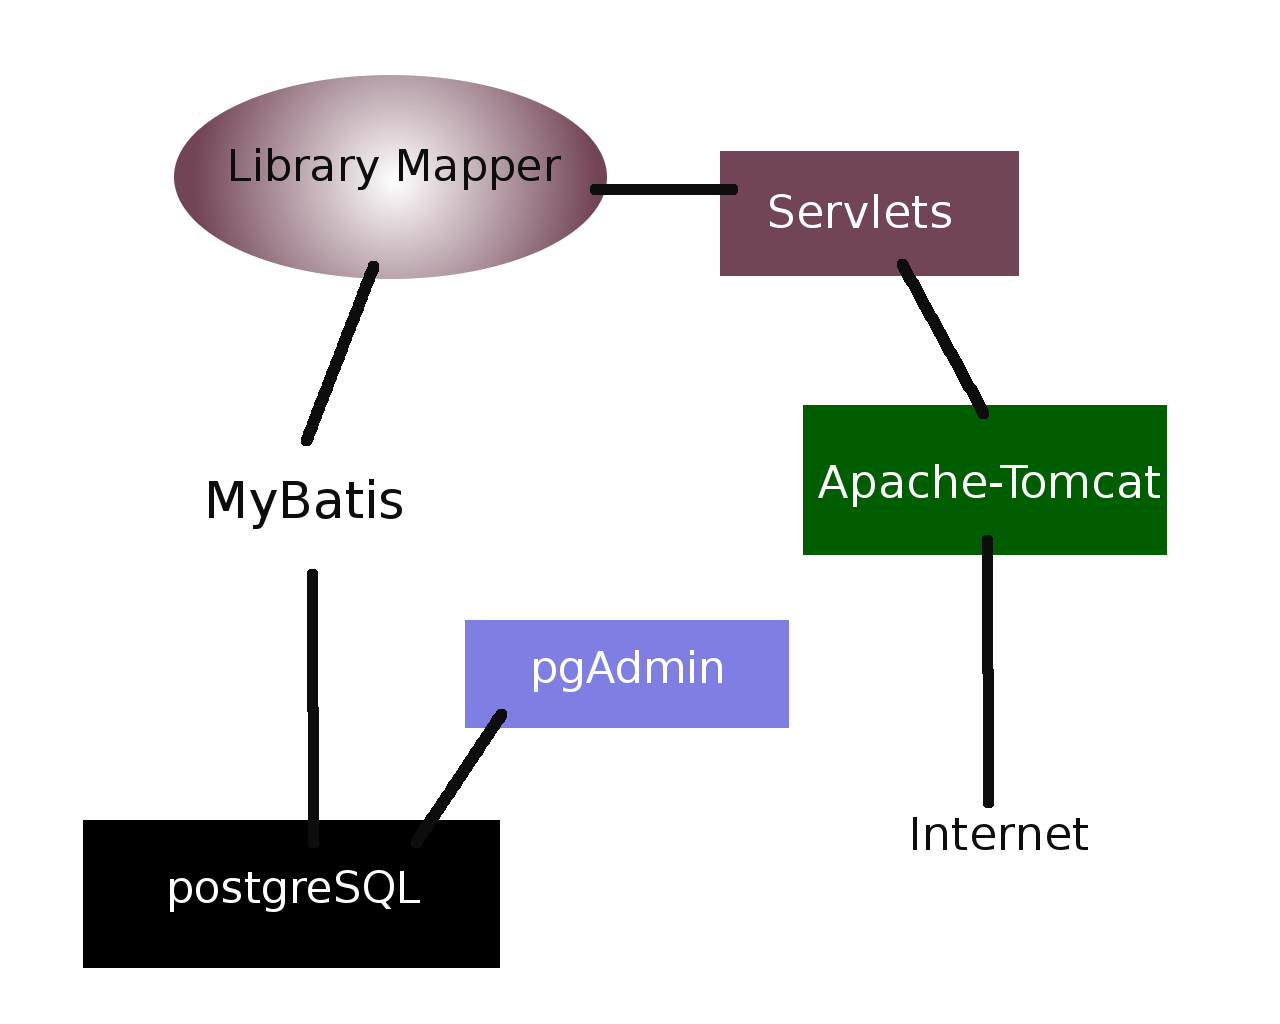
\includegraphics[width=0.70\textwidth]{./imgs/esquemaLibrary.png}
	\caption{Técnologias usadas}
	
      \end{figure}

	
      \subsubsection{O que são Qr-Codes?}
      Quick Response Code foi inventado por \href{http://www.denso-wave.com/}{DENSO WAVE}, uma empresa Japonesa de captura automática de dados, FA e campos de solução de negócios, em 1994 e foi um dos primeiros códigos de barra 2D
      a ser usado em aplicações onde era necessário uma combinação de camera de aparelhos celulares e códigos de barra 2D.\cite{barcode}Esses códigos trocam barras e espaços
      por pontos e espaços arranjados num vetor ou uma matrix, aumentando consideravelmente a quantidade de dados
      armazenados num espaço igualmente usado para um código de barra 1D.\\

      Apenas em 2002 cameras de celulares foram comercialmente vendidas com dispositivos reconhecedores de Qr-codes e desde
      então uma vasta variedade de aplicativos começou a surgir no Japão e vem tomando o mundo.
	\begin{figure}[H]
	\centering

      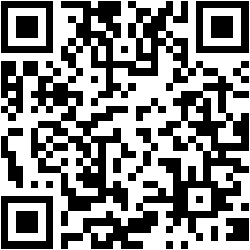
\includegraphics[width=0.20\textwidth]{./imgs/qrcode.png} 
      \end{figure}
	Em 2006, como parte do Windows Live service, a Microsoft lançou o Windows Live Barcode
      , onde Qr-codes eram usados como ponte para troca de informações entre aparelhos mobile e outras medias como PCs, Tv de plasma
      e revistas.\\
      
      As Qr-Codes geradas para esse projeto passarão para o usuário o endereço de uma página web de busca dos livros da 
      bilioteca em que ele se encontra.Junto nessa URL tem um id do Qr-Code, que mostra para o programa onde no grafo
      do mapa da biblioteca se encontra o visitante, para dessa maneira poder criar o caminho que o mesmo deve traçar.\\
      
      
      
      \subsubsection{Grid Graphs}
      
      Um grafo \textit{G} é uma par \textit{(V,E)}, onde \textit{V} é um conjunto finito e \textit{E} é uma relação binária de \textit{V}.
      O conjunto \textit{V} é chamado de o \textit{conjunto de vértices} de \textit{G} e seus elementos são chamados 
      de \textit{vértices}.O conjunto \textit{E} é chamado de \textit{conjunto de arestas} de \textit{G} e seus elementos
      são chamados de \textit{arestas}.Existem dois tipos de grafos - grafo direcionados e grafos não-direcionados.
            \cite{bfs}\\
      
      Uma aresta num \textit{grafo não-direcionado} é um conjunto \textit{\{u,v\}} onde \textit{u,v} $\in$ \textit{V} e \textit{u $\neq$ v} que por
      convenção é definida como \textit{$(u,v)$} ou \textit{$(v,u)$} e é possível ir de \textit{u} para \textit{v} e de \textit{v} 
      para \textit{u}.\\
      
      Já num \textit{grafo direcionado} (ou \textit{dígrafo} ) uma aresta é identificada por setas e \textit{$(u,v)$} \textit{$\neq$} \textit{$(v,u)$}.
      
     \begin{figure}[H]
	\centering
      	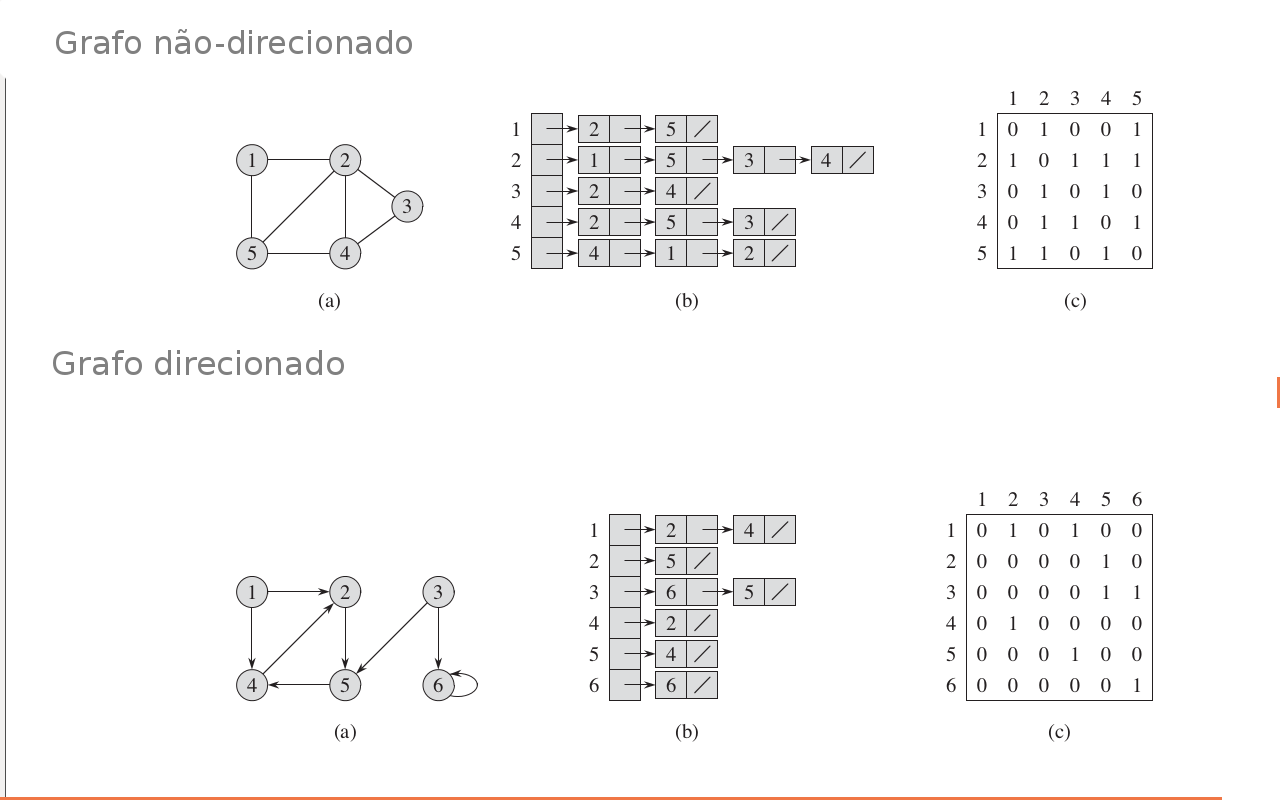
\includegraphics[width=0.7\textwidth]{./imgs/grafo.png}\\[1cm]
      	\caption{Grafo retirado do livro \cite{bfs}}
      \end{figure}
      Em ambos os casos uma aresta \textit{(u,v)} pode possuir um \textit{peso} que indica o custo por passar do vértice \textit{u}
      para o \textit{v}.\\
      
      Um Grid Graph ( grafo do tipo Grid ) é um grafo não-direcionado; uma grade de nós (vértices) \textit{n} x \textit{n} sendo que cada
      nó tem exatamente 4 arestas com exceção dos nós das extremidades.
       \begin{figure}[H]
	\centering
      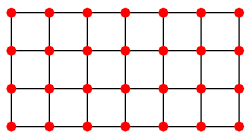
\includegraphics[width=0.5\textwidth]{./imgs/grid.png}\\[1cm]
	\caption{Representação de um Grid}
      \end{figure}
      Para o LibraryMapper será usado um grafo não-direcinado do tipo Grid alocado numa matriz, sendo que cada vértice do grafo 
      será um nó da classe Node.Essa Possui os seguintes atributos:\\
      
      
      \begin{lstlisting}
package library.domain;

public class Node {
    
    private Integer idNode;
    private Integer positionX;
    private Integer positionY;
    private Integer contentId;
    private Integer idLibrary;
    private String codeIdInitialShelf;
    private String codeIdFinalShelf;t
    private String contentType;//Free,QrCode,Forbidden,Shelf
    private Node parentFromBeginNode;
    private Node parentFromEndNode;
    public int isInUse;
    private Semaphore semaphore;
    private String color;
    private String whoMarkedThisNode;
/*... continua ...*/
\end{lstlisting}
\vspace{1cm}
{\bf idNode:} o id de cada novo Node. \\
{\bf positionX: }coluna j na matriz Mapa(i,j)\footnote{A matriz que se refere ao mapa da biblioteca}      . \\
{\bf positionY: }linha i na matriz Mapa(i,j).\\
{\bf contentsType:} Tipo do Node, podendo variar entre Free, Forbidden, QrCode ou Shelf.\\
{\bf contentsId: }Uma vez definido qual o tipo do Node é necessário saber qual o seu id na tabela relacionada.Caso não possua uam tabela, como é o caso
 de Free e Forbidden, o ContentsId é um valor desnecessário\\
{\bf idLibrary:} o id da biblioteca a qual pertence.\\
{\bf codeIdInitialShelf: }o identificador inicial de uma estante\\
{\bf codeIdFinalShelf:}o identificador final de uma estante\\
{\bf parentFromBeginNode:}o nó pai do nó atual na busca feita partindo do ponto inicial definido \\
{\bf parentFromEndNode:}o nó pai do nó atual na busca feita partindo do ponto final definido\\
{\bf isInUse:}flag que define se o nó em questão está sendo usado por outro processo de busca.\\
{\bf semaphore:} semáforo do nó.\\
{\bf color:} cor do nó definida no esquema da BFS.\\
{\bf whoMarkedThisNode:} valor que define qual busca já passou por esse nó.\\


      Alguns atributos serão melhores descritos nas próximas seções.\\
      
      
      \subsubsection{Breadth-First Search (BFS)}
      Dado um grafo \textit{G=(V,E)} com um vértice \textit{s} distinto, Breadth-first search explora sistematicamente
      as arestas de \textit{G} para descobrir todo vértice que pode ser alcançado por \textit{s}.Ele computa a distância
      (menor número de arestas) do vértice \textit{s} até todos os vértices que ele possa alcançar.Para manter o controle do progresso da busca, BFS procura cores em cada vértice - branco, cinza e preto. Todos os 
      vértices começam com cor branca, eventualmente passam para cinza e por fim  ficam pretos.\cite{bfs}\\
      
      Uma vez que um vértice é descoberto ele se torna não-branco.Um vértice só se tornará preto quando todos os vértices
      que são adjacentes á ele tenham sido descobertos, enquanto isso ele será cinza.Isso representa a fronteira entre
      vértices descobertos e não-descobertos como mostrado na Figura~\ref{./imgs/bfs.png}\\
	
	Como no pior caso, a busca tem que ser feita em todos os (m) nós de um grafo e passar por todas suas (a) arestas.Como a 
      BFS não volta nos caminhos que já traçou, a complexidade desse algoritmo é O(a).\\	 
      \begin{figure}[H]
	\centering
      	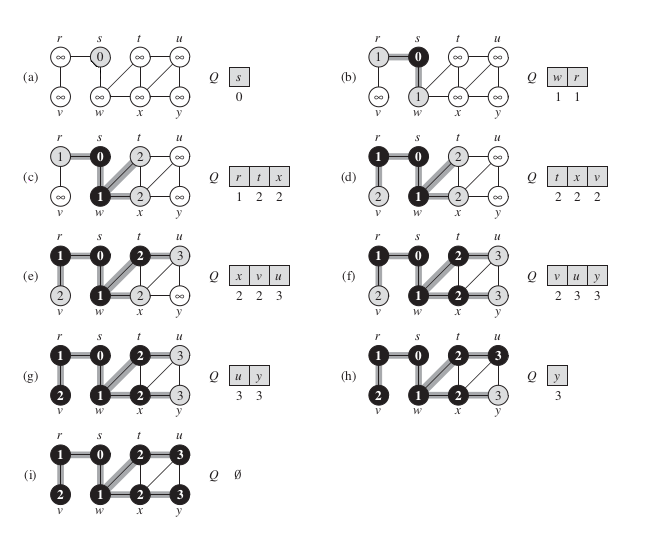
\includegraphics[width=0.50\textwidth]{./imgs/bfs.png}
	\caption{BFS retirada do livro \cite{bfs}}
	\label{./imgs/bfs.png}
      \end{figure}
      Além das cores, nesse projeto essa BFS distingue entre nós (vértices) do tipo Free, Bookshelf, Qr-Code e Forbidden e será 
      aplicada de uma maneira Bi-direcional.\\
      
      \subsubsection{Bi-directional BFS}
	A idéia por trás de uma busca Bi-direcional é fazer duas buscas rodarem simultaneamente - Uma "para frente", 	 
	saindo do estado inicial (a origem) da busca inteira e outra "para trás",  saindo do estado final ( a chegada ) 
	da busca inteira esperando que ambas se encotrem no meio.\cite{bidirecional}. 
 	\begin{figure}[H]
	\centering
	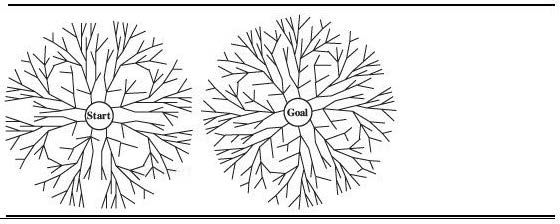
\includegraphics[width=0.8\textwidth]{./imgs/bi-directional.png}\\[1cm]   
	\caption{BFS bi-direcional retirada do livro \cite{bidirecional}}
      	\end{figure}
	Nesse projeto a busca Bi-direcional será realizada através de métodos concorrentes de programação.Cada pólo
	iniciará sua busca paralelamente liberando assim duas threads.Caso uma thread chegue em um nó que já foi 
	visitado ela define aquele nó como o "meio do caminho" e a partir dele gera a rota inteira do mapa.Mas caso o nó que
	chegue esteja sendo visitado, ela para e abandona o que estiver fazendo para depois ser reciclada num outro novo processo.
	Nas próximas seções serão demonstradas com maiores detalhes, como essa busca foi implementada no Library Mapper.\\
 
	Pela profundidade da busca ter caído pela metade, ou seja, no máximo uma busca tem que ir até a metade do grafo, a 
	complexidade do algoritmo é O(a/2).\\
	

	
	
	\subsubsection{pgAdmin - Interface gráfica para gerenciamento do banco de dados PostgreSQL}
	{\it	pgAdmin é o recurso de administração Open-Source para o banco de dados PostgreSQL. O aplicativo 
	pode ser usado no Linux, FreeBSD, Solaris, Mac OSX e Windows para gerenciar o PostgreSQL 7.3 e acima executado em qualquer
	 plataforma, bem como versões comerciais e derivados do PostgreSQL como Postgres Plus avançado Server e banco de dados Greenplum.\\
	
	pgAdmin é projetado para atender as necessidades de todos os usuários, desde escrever consultas SQL simples para o 
	desenvolvimento de bancos de dados complexos. A interface gráfica suporta todos os recursos do PostgreSQL e facilita
	 a administração. O aplicativo também inclui um destaque de sintaxe SQL editor, um editor de código do lado do servidor, 
	um agente de agendamento de tarefas SQL/batch/shell,etc. Conexão com o servidor pode ser feita usando TCP / IP ou soquetes
	 de domínio Unix (nas plataformas * nix), e pode ser criptografado SSL para a segurança. Drivers adicionais não são necessários
	 para se comunicar com o servidor de banco de dados.}\cite{pgAdmin}\\

	
	Com o pgAdmin não é possível iniciar um servidor de Banco de dados no linux. É necessário um terminal para criar
	 e configurar um servidor de banco de dados e referenciá-lo no pgAdmin.Contudo uma vez isso feito, fica fácil
	 criar banco de dados e também editar, deletar tabelas e colunas desse banco.Como exemplo, a figura \ref{telaPgAdmin} mostra como 
	é a tela de administração dos bancos de dados em conjunto de uma das tabelas do banco do Library Mapper.\\ 
	
	No Library Mapper foi criado um banco de dados com o nome libraryMapperBD que utiliza a porta padrão do servidor de dados para se comunicar com o programa.
	Os detalhes desse banco serão vistos logo em seguida.\\

	\subsubsection{PostgreSQL}
	{\it O PostgreSQL é um poderoso sistema gerenciador de banco de dados objeto-relacional de código aberto.  
	Tem mais de 15 anos de desenvolvimento ativo e uma arquitetura que comprovadamente ganhou forte reputação 
	de confiabilidade, integridade de dados e conformidade a padrões.  Roda em todos os grandes sistemas operacionais, 
	incluindo GNU/Linux, Unix (AIX, BSD, HP-UX, SGI IRIX, Mac OS X, Solaris, Tru64), e MS Windows. É totalmente compatível
	 com ACID, tem suporte completo a chaves estrangeiras, junções (JOINs), visões, gatilhos e procedimentos armazenados
	 (em múltiplas linguagens).  Inclui a maior parte dos tipos de dados do ISO SQL:1999, incluindo INTEGER, NUMERIC, BOOLEAN, 
	CHAR, VARCHAR, DATE, INTERVAL, e TIMESTAMP.  Suporta também o armazenamento de objetos binários, incluindo figuras, sons ou
	 vídeos.  Possui interfaces nativas de programação para C/C++, Java, .Net, Perl, Python, Ruby, Tcl, ODBC, entre outros, e 
	uma excepcional documentação.}


	\begin{figure}[H]
	\centering
	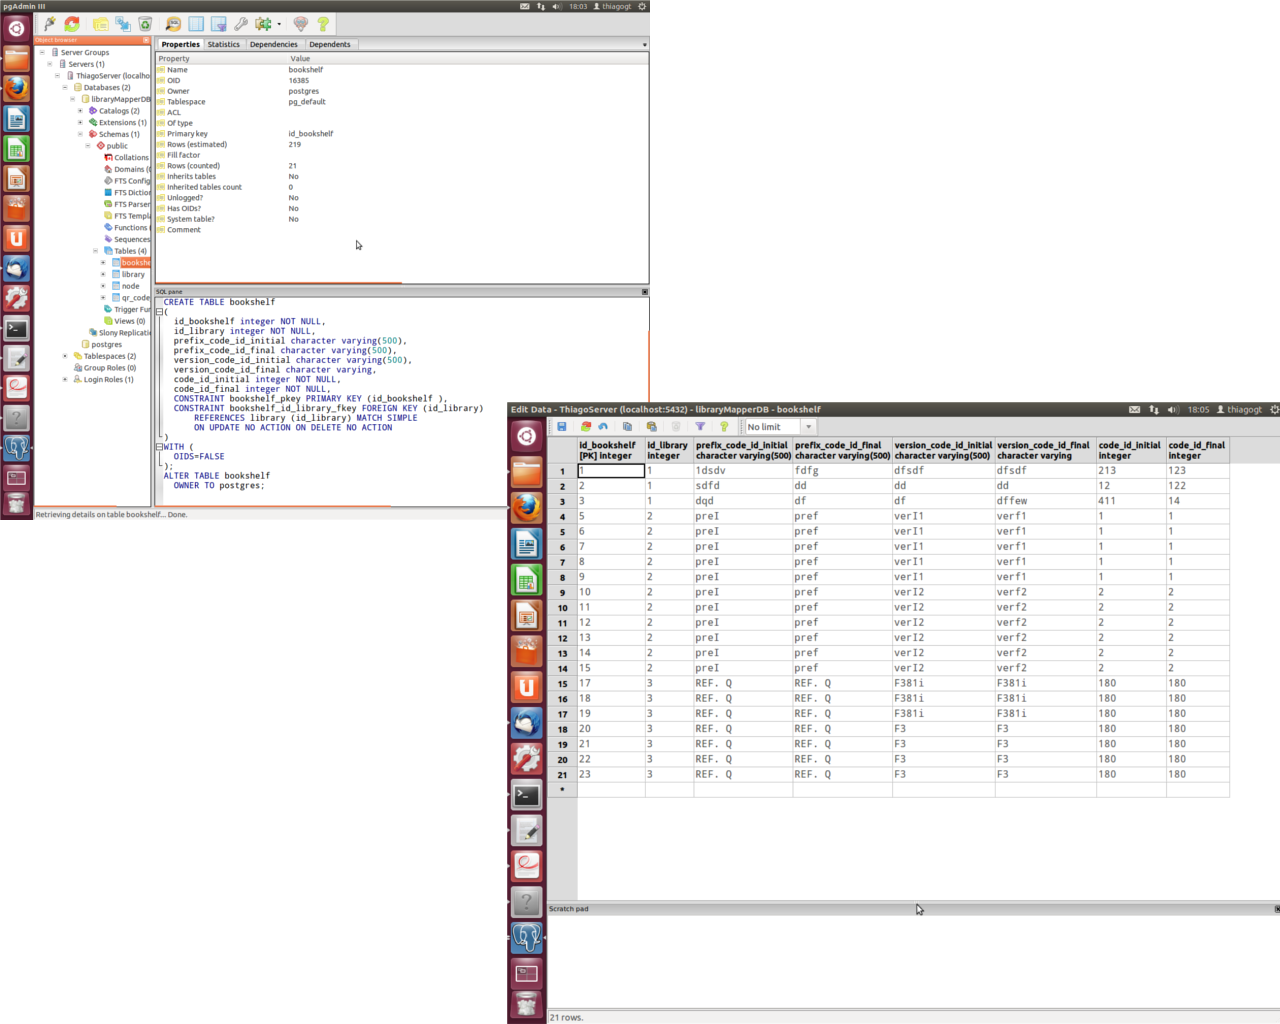
\includegraphics[width=0.87\textwidth]{./imgs/pgAdminLibrary.png}\\[1cm]   
	\caption{tela de administração pgAdmin e tabela de dados}
	\label{telaPgAdmin}
      	\end{figure}
		
	{\it Como um banco de dados de nível corporativo, o PostgreSQL  possui funcionalidades sofisticadas como o controle de concorrência 
	multiversionado (MVCC, em inglês), recuperação em um ponto no tempo (PITR em inglês), tablespaces, replicação assíncrona, transações
	 agrupadas (savepoints), cópias de segurança a quente (online/hot backup), um sofisticado planejador de consultas (otimizador) e registrador 
	de transações sequencial (WAL) para tolerância a falhas.  Suporta conjuntos de caracteres internacionais, codificação de caracteres multibyte, 
	Unicode e sua ordenação por localização, sensibilidade a caixa (maiúsculas e minúsculas) e formatação.  É altamente escalável, tanto na quantidade
	 enorme de dados que pode gerenciar, quanto no número de usuários concorrentes que pode acomodar. Existem sistemas ativos com o PostgreSQL em
	 ambiente de produção que gerenciam mais de 4TB de dados.  Alguns limites do PostgreSQL estão incluídos na tabela abaixo.}\cite{postgresql}
	
	\begin{table}[H]
 	\centering
	\begin{tabular}{|l|c|} \hline
		Tamanho Máximo do Banco de Dados &  ilimitado\\ \hline
		Tamanho máximo de uma Tabela  &	32 TB\\ \hline
		Tamanho Máximo de uma Linha &	1.6 TB\\ \hline
		Tamanho Máximo de um Campo  & 	1 GB\\ \hline
		Máximo de Linhas por Tabela &	Ilimitado\\ \hline
		Máximo de Colunas por Tabela & 	250–1600 dependendo do tipo de coluna\\ \hline
Máximo de Índices por Tabela & 	Ilimitado\\ \hline
	\end{tabular}
	\caption{Dados retirados do site \href{http://www.postgresql.org.br/sobre}{PostgreSQL}}
	\label{t_fixa}
\end{table}	
	O banco de dados usado pelo Library Mapper é criado para armazenar a matriz que se refere ao mapa da biblioteca, 
	representada aqui por Mapa(i,j).\\O banco contém 4 tabelas:
\begin{itemize}
\item{library}\\[0.3cm]
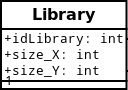
\includegraphics[width=0.20\textwidth]{./imgs/librayBD.png} 

Essa tabela foi criada para o cliente ter liberdade de criar inúmeras versões de bibliotecas e também carregá-las quando queira.\\

idLibrary: o id de cada nova biblioteca criada.\\
size\_X: número de colunas na matriz Mapa(i,j).\\
size\_Y: número de linhas na matriz Mapa(i,j).\\


\item{node}\\[0.3cm]	
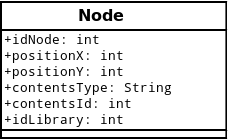
\includegraphics[width=0.30\textwidth]{./imgs/nodeBD.png}\\

Cada Node equivale a uma posição na matriz Mapa(i,j)

idNode: o id de cada novo Node. \\
positionX: coluna j na matriz Mapa(i,j). \\
positionY: linha i na matriz Mapa(i,j).\\
contentsType: Tipo do Node, podendo variar entre Free, Forbidden, QrCode ou Shelf.\\
contentsId: Uma vez definido qual o tipo do Node é necessário saber qual o seu id na tabela relacionada.Caso não possua uam tabela, como é o caso
 de Free e Forbidden, o ContentsId é um valor desnecessário\\
idLibrary: o id da biblioteca a qual pertence.\\\\

\item{bookshelf}\\[0.3cm]
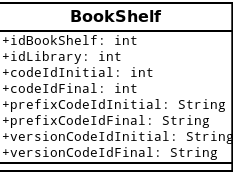
\includegraphics[width=0.30\textwidth]{./imgs/bookShelfBD.png}\\	

Quando uma bookshelf é criada ela recebe dois identificadores, sendo um referente ao primeiro livro contido nela e o outro o último.Dessa maneira, é possível
identificar o range de livros contido nela.Mas para ser possível fazer uma busca no banco de dados nesse range, é necessário retirar dois
valores inteiros, sendo um o início e o outro o fim do range.Por isso a tabela bookshelf divide os identificadores em 3 partes: prefixo ,codeId
e versão.Dessa maneira, com a identificação do prefixo mais a verificação no range da estante, é possível retornar uma consulta precisa da estante
que se encontra o livro.A figura \ref{parser} mostra a maneira como uma das duas indentificações é dividida para ser guardada no banco de dados.
\begin{figure}[H]
	\centering
	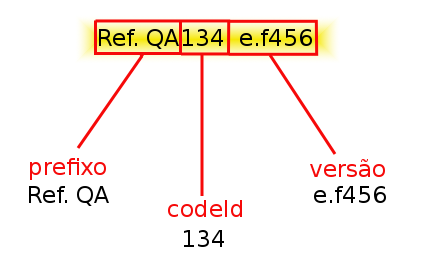
\includegraphics[width=0.40\textwidth]{./imgs/estanteParseada.png}\\[1cm]   
	\caption{Identificação da estante parseada.}
	\label{parser}
\end{figure}

idBookShelf: o  id de cada nova estante\\
idLibrary: o id da biblioteca a qual pertence.\\
prefixCodeIdInitial: prefixo incial da estante\\
codeIdInitial:range inicial da estante\\
versionCodeIdInitial:versão inicial da estante\\
prefixCodeIdFinal:prefixo final da estante\\
codeIdFinal:range final da estante\\
versionCodeIdFinal:versão final da estante
\item{qr\_cod\_mark}\\[0.3cm]

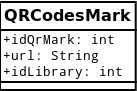
\includegraphics[width=0.20\textwidth]{./imgs/qrCodeBD.png}\\	

idQrMark: id de cada novo QrCode\\
url: a url contida no QrCode.\\
idLibrary:o id da biblioteca a qual esse QrCode pertence\\
\end{itemize}
	A imagem abaixo ilustra o banco de dados completo.
\begin{figure}[H]
	\centering

	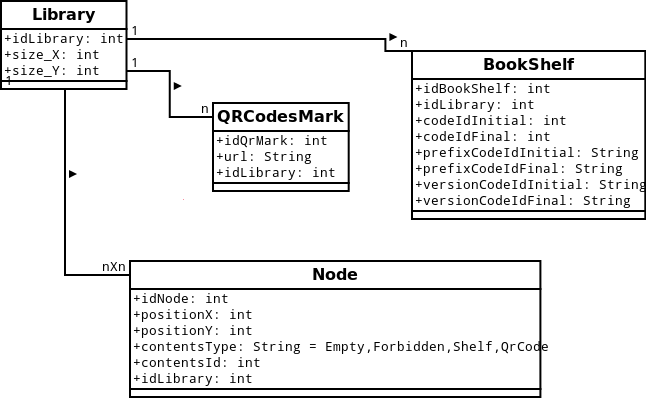
\includegraphics[width=0.70\textwidth]{./imgs/merLibraryMappper.png}\\[1cm]	
	\caption{Identificação da estante parseada.}
	\label{total}
\end{figure}

	\subsubsection{Mybatis - Mapeando SQL para JAVA}
	
	Uma vez criado o banco de dados, é necessário criar métodos que permitam operar nesse BD.Contudo, para isso ser possível
	é necessário fazer consultas em SQL no BD da aplicação, a qual está toda escrita em linguagem JAVA.Isso não é um grande 
	problema, mas consome tempo e pasciência do programador que terá que fazer vários ajustes e códigos extras em JDBC.
	(JDBC ou Java Database Connectivity é um conjunto de Classes e interfaces em JAVA, que conversam com qualquer Banco de dados através 
	de envio de intruções SQL.)
	
	{\it MyBatis é um framework de persistência de primeira classe, com 
	suporte para SQL personalizado, procedimentos armazenados e mapeamentos avançados. 
	MyBatis elimina quase todo o código JDBC e ajuste manual dos parâmetros e recuperação 
	de resultados. MyBatis pode usar XML simples ou Anotações para configuração e mapa primitivas,
	 interfaces e POJOs Mapa Java (Plain Old Java Objects) para registros de dados.}\cite{mybatis}\\

	No Library Mapper ainda foi usado uma ferramenta do Eclipse chamada {\it MyBatis Generator} que monta todo o mapeamento 
	feito pelo Mybatis direto no projeto.Ao configurar dois arquivos, generatorConfig.xml e MapperConfig.xml, setando quais as
	tabelas deveriam ser mapeadas para suas futuras classes no Library Mapper, tudo é gerado automaticamente pela ferramenta.\\

	O mapeamento consiste em três partes:\\
	\begin{itemize}
	\item{As Classes Domínio}\\
	Essas são as classes correspondentes aos atributos do Banco de Dados.Necessariamente todas as colunas de um BD têm 
	que estar relacionadas a um atributo dessas classes, mas o contrário não é verdade.Quando um select é feito com as interfaces Mapas
	descritas abaixo, um objeto de um dos domínios é retornado.\\

	Library.java, BookShelf.java, Node.java e QrCodeMark.java são as classes domínio no Library Mapper.\\

	\item{As interfaces Mapas}\\
	Essas são as interfaces JAVA com o métodos de consultas SQL e são elas que serão usadas pelo programador para fazer uma consulta
	no banco de dados.Essas interfaces chamam os métodos implementados nos XMLs, descritos abaixo.\\
		
	LibraryMapper.java, BookShelfMapper.java, NodeMapper.java e QrCodeMarkMapper.java são as interface Mapas no Library Mapper.\\
	\item{Os XMLs}\\
	Essas são as consultas com linguagem parcialmente SQL.Essas são as consultas mais próximas a uma linguagem SQL e são elas que são
	usadas nos Bancos de Dados.Todas as consultas desses arquivos têm o mesmo nome que os métodos das interfaces Mapas.\\

	LibraryMapper.xml, BookShelfMapper.xml, NodeMapper.xml e QrCodeMarkMapper.xml são os XMLs de consulta do Library Mapper.\\
	\end{itemize}
	
	Uma vez gerado todo o mapeamento, basta criar uma nova seção e começar a usar os métodos da interface Mapas.
	

	\subsubsection{JSP, Servlets e Apache Tomcat}


	{\it A tecnologia JavaServer Pages (JSP) permite que os desenvolvedores da Web e
	 designers desenvolvam e mantenham de uma maneira fácil e rápida páginas Web dinâmicas 
	. Como parte da família da tecnologia Java, a tecnologia JSP permite o rápido desenvolvimento
	 de aplicações baseadas na Web que são independentes de plataforma. A tecnologia JSP separa
	 a interface do usuário a partir de geração de conteúdo, permitindo aos designers para alterar
	 o layout geral da página sem alterar o conteúdo dinâmico subjacente. JavaServer Pages é uma extensão 
	da tecnologia Java Servlet.\\
	
	 Servlets são independentes de plataformas, são módulos que se encaixam perfeitamente em 
	uma estrutura de servidor Web e podem ser usados para estender
	 as capacidades de um servidor Web com mínima sobrecarga, manutenção e suporte. Ao contrário de outras linguagens de
	 script, servlets não envolvem nenhuma consideração específica da plataforma ou modificações, que são componentes de
	 aplicativos que são baixados, a pedido, para a parte do sistema que precisa deles.}\cite{jsp}\\

	Apache Tomcat é uma implementação open source do Java Servlet e JavaServer Pages, responsável por manter as páginas do Library Mapper
	na internet.
	
	\subsubsection{JSF2 - Managed Beans}
	O JavaService Facelets 2 oferece muitos recursos para o desenvolvimento de uma aplicação Web Java, sendo um dos principais os Managed Beans que são
	objetos utilizados para:
		{\it\begin{itemize}
	\item{Receber os dados enviados pelos usuários através das telas Web da aplicação.}
	\item{Executar as lógicas para tratar as requisições dos usuários.}
	\item{Disponibilizar os dados que devem ser apresentados nas telas da aplicação Web.}\cite{k19}	 	
	\end{itemize}}
	
	No Library Mapper existe dois grandes Managed Beans que cuidam das interfaces Web, o MapBean.java e o SearchBean.java, sendo que o 
	primeiro é responsável por toda a parte de criação da biblioteca e o segundo por todo o processo de busca, desde a requisição ao 
	Colméia até a geração do Mapa com o caminho.
	
	\subsubsection{JavaScript, jQuery e JSON}
	 JavaScript é uma linguagem de script baseada no padrão ECMAScript, aprovado como um padrão internacional ISO/IEC 16262, em abril de 1998,
	 utilizada para programação client-side em navegadores web.Foi inventada por Brendan Eich na Netscape e primeiro
	apareceu no navegador Navigator 2,0 da empresa . Ele já apareceu em todos os browsers Netscape subseqüentes e em todos os navegadores da Microsoft começando com Internet Explorer 
	3.0.\cite{javascript}\\

	{\it jQuery é uma biblioteca JavaScript rápida e concisa que simplifica num documento HTML o tratamento da manipulação de eventos, animação
	 e interações Ajax para desenvolvimento web rápido.}\cite{jquery} \\
	
	JSON {\it (JavaScript Object Notation) é um formato de troca de dados leve. É fácil para os seres humanos
	 lerem e escreverem. É fácil para máquinas para analisar e gerar. É baseado em um subconjunto da linguagem de programação
	 JavaScript. JSON é um formato de texto que é completamente independente
	 do idioma, mas usa convenções que são familiares aos programadores da família-C de línguas, incluindo C, C + +, C \#, Java,
	 JavaScript, Perl, Python, e muitos outros. Essas propriedades fazem JSON uma linguagem de troca de dados ideal.}\cite{JSON}\\


	No Library Mapper o javaScript foi usado para criar métodos que ajudassem na lógica das interfaces e também para criar objetos
	semelhantes aos usados na parte JAVA, como no caso das estantes, qrCode e blocos livres e proibidos ao usuário passar.\\
	 
	O jQuery teve papel fundamental na parte responsável pela edição via Web do mapa da bilbioteca.Métodos como {\it resize}, {\it drag} e {\it drop}
	foram utilizados para possibilitar que um desses objetos javaScript descritos anteriormente se tornassem modeláveis através da interface Web.\\     

	O JSON foi responsável por fazer a conversão dos objetos criados na interface Web em um parâmetro compreensível para o Libray Mapper.
	\subsubsection{HTML5 - Canvas}
	{\it Hypertext Markup Language ou HTML é a linguagem de publicação da World Wide Web.}\cite{html}Atualmente na versão 5, o HTML
	possui novas funcionalidades e consegue realizar tarefas que antes só conseguia realizar através de outras ferramentas, como por exemplo
	carregar arquivos locais.\\

	Funcionando como um conteiner de processamento gráfico (gráfico de jogos, arte ou imagens) provê scripts para a renderização desses gráficos.
	Pode gerar qualquer tipo de forma, com qualquer tipo de cor, textura, etc e por isso, no Library Mapper é usado para gerar os mapas
	já com os caminhos mapeados, para o visitante que procuram por um livro.\\

	A classe responsável por esse script canvas é a CanvasMap.java que divide a criação do mapa em duas partes: Uma do carregamento do mapa
	 sem o caminho traçado da busca e outra para o desenho do resultado da busca.O primeiro caso é resolvido pelo método {\it loadNodesFromBD(StringBuilder out)} que verifica se
	a matriz Mapa(i,j) já foi carregada pelo Library Mapper, carregando ou não do banco de dados (dependendo da resposta) e transformando cada Node
	dessa matriz num quadrado colorido no mapa mostrado ao usuário.O parametro {\it out} passado é uma StringBuilder do JAVA, responsável por guardar o que será escrito no arquivo do mapa desenhado .xhtml.\\

	O segundo caso é resolvido pelo método {\it loadSearch(StringBuilder out, Book selectedBook)} que fica  responsável por extrair as posições de saída (QrCode - retirado da URL que iniciou a seção) e chegada (estante do livro - retirada do livro {\it selectedBook}) da procura pelo livro e por chamar a busca dessas posições.


      	\subsubsection{Desenvolvimento mobile}
	{\it As pessoas apreciam aplicativos iOS que sentem como se eles fossem projetados especificamente para o dispositivo. Por exemplo, quando um aplicativo se encaixa bem na tela do dispositivo e responde aos gestos que as pessoas conhecem, que fornece grande parte da experiência as quais as pessoas estão procurando. E, embora as pessoas possam não estar cientes dos princípios de design de interface humana, como a manipulação direta ou consistência, esses usuários podem dizer quando os aplicativos seguem esses princípios e quando não.Ao começar a projetar um aplicativo iOS, certifique-se de compreender e aprender como incorporar os princípios de design HI de modo que você possa oferecer ao usuário uma experiência pessoal que ele irá apreciar.}\cite{mobile}\\

	Inicialmente o Library Mapper foi desenvolvido apenas para se encaixar nos padrões IOS, especificamente para iPhones.Por isso toda sua interface e a maneira como o usuário opera o Library Mapper foi pensada para proporcionar uma experiência rápida e de fácil compreensão.Um exemplo é a página inicial de busca semelhante a usada pelo Google, que permite que o usuário reconheça facilmente que se trata de uma página de busca, pois já está familiarizado com o padrão.Outro exemplo é a idéia de um mapa ao invés de coordenadas descritivas como vire a esquerda na estante x, depois a direita, etc.Os botões estilizados para o toque e a lista de livros ocupando a tela inteira são outros exemplos também.
	\subsubsection{Integração Contínua}
	{\it	Integração Contínua é uma prática de desenvolvimento de software onde os membros de uma equipe integram seu trabalho frequentemente, geralmente cada pessoa integra pelo menos diariamente - levando a múltiplas integrações por dia. Cada integração é verificada por uma compilação automatizada (incluindo teste) para detectar erros de integração, o mais rapidamente possível.}\cite{ic}\\

	Por mais estranho que pareça falar de Integração Contínua para um time de uma única pessoa, chegou um ponto durante a criação do Library Mapper que essa técnica, ou parte dela, tornou-se essencial pois eu estava trabalhando nele em 3 lugares diferentes, com horários completamente diferentes de um dia para outro.Comecei a comitar tudo que eu fazia, indiferente se estava certo ou errado, pois assim conseguia continuar do ponto certo de onde parei.Também comecei a me policiar a tentar comitar algo todo dia, porque estava com o tempo muito restrito para desenvolver o projeto, afinal tinha que diviví-lo entre trabalho, casa recém comprada, faculdade e médico para meu futuro filho. 	   
   \subsection{Library Mapper, o cliente}
	Essa seção é reservada para explicar toda a parte relacionada ao cliente da aplicação e, nesse caso, o cliente é o responsável pela biblioteca.O único trabalho desse cliente é montar a biblioteca pela interface Web, identificando cada estante corretamente e onde ficarão os QR-Codes.
	Nessa primeira versão do Library Mapper, os qr-codes criados no programa são armazenados no banco de dados da aplicação e não há como identificá-los sem ter que olhar no BD pela ordem que foram criados.
	\subsubsection{Construindo o seu mapa Web} 
	
		Para a construção do mapa da biblioteca para o Library Mapper, existe uma interface Web que auxilia todo o processo de construção e identificação das estantes.Acessando http://host/LibraryMapper/faces/WebLibraryMapper/mapCreation.xhtml uma tela com um espaço definido para construção junto de todos acessórios para montagem do mapa aparecerão, como mostrado na figura  \ref{mapCreation}.\\

	Desses acessórios existe um botão Save para salvar o mapa no Banco de dados e quatro objetos para montagem da biblioteca:
\begin{figure}[H]
	\centering
	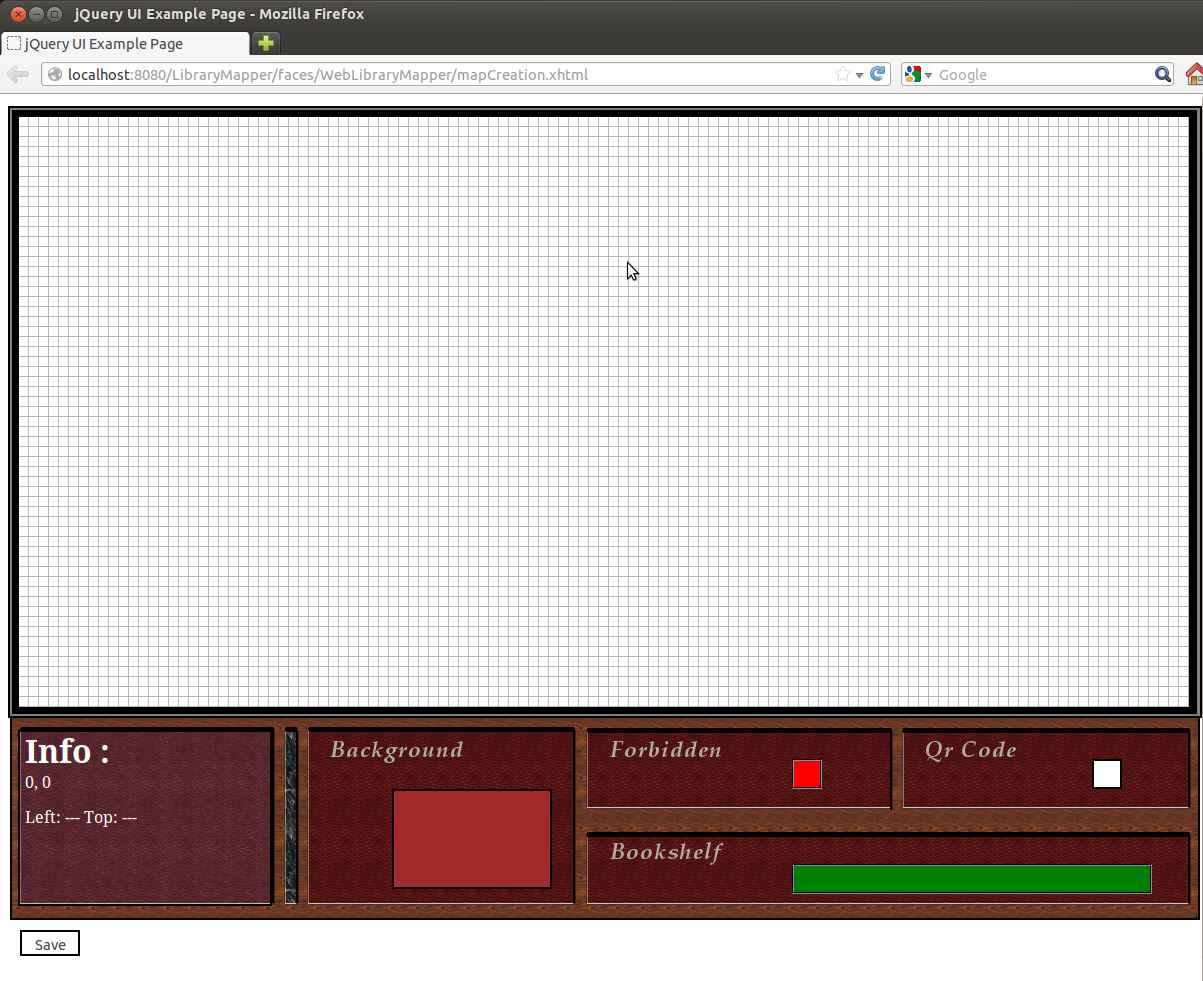
\includegraphics[width=0.95\textwidth]{./imgs/mapCreation.png}\\[1cm]   
	\caption{Interface Web para criação de mapas.}
	\label{mapCreation}
\end{figure}	

\begin{itemize}	
	\item{{\bf Background  }}\\
		O objeto background deve ser utilizado para montar o chão da biblioteca, ou seja, é a base da biblioteca e tudo deve ser montado em cima dele.Uma vez o mapa transformado na matriz utilizada pelo Library Mapper, a parte do Background que não possua nada em cima será definida como um Node do tipo Free. 	
	\item{{\bf Qr Code  }}\\	
		O objeto Qr Code deve ser colocado na mesma posição onde será colocado na biblioteca física, pois senão o usuário encontrará problemas para se orientar no mapa.Uma vez o mapa transformado na matriz utilizada pelo Library Mapper, cada parte do QrCode gerado será um Node do tipo QrCode. 	
	\item{{\bf Forbidden  }}\\
		O objeto Forbidden deve ser enterpretado, com exceção das estantes, como qualquer obstáculo existente na biblioteca: vasos, colunas, esculturas, ou seja, qualquer coisa que impeça o usuário de passar por aquele espaço específico.Uma vez o mapa transformado na matriz utilizada pelo Library Mapper, cada parte do Forbidden gerado será um Node do tipo Forbidden.	
	\item{{\bf BookShelf }}\\
		O objeto BookShelf deve ser enterpretado como {\bf uma parte da estante} física, ou a estante inteira, dependendo dos livros que ela possui.Uma estante é definida por dois identificadores, sendo um de início referente ao primeiro livro da estante e um de fim, referente ao último livro da estante.No caso da biblioteca do IME-USP a identificação é feita dessa maneira e começa no topo esquerdo da estante e termina no piso direito da mesma, como mostrado na figura \ref{estante}.
\begin{figure}[H]
	\centering
	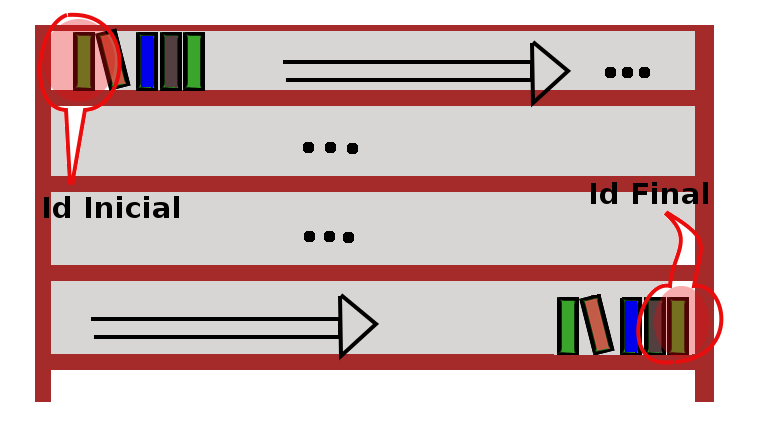
\includegraphics[width=0.60\textwidth]{./imgs/estanteIME.png}\\[1cm]   
	\caption{Referencia a organização de uma estante na biblioteca IME-USP}
	\label{estante}
\end{figure}

Caso uma estante seja um conjunto de livros do mesmo prefixo, então tem-se uma estante inteira igual a estante física como na figura \ref{variasEstantes}.b, porém caso existam vários tipos de conjuntos de prefixos devem ser criadas n estantes do Library Mapper, onde n é o número de conjuntos contidos na estante física, como mostrado na figura \ref{variasEstantes}.a.
\begin{figure}[H]
	\centering
	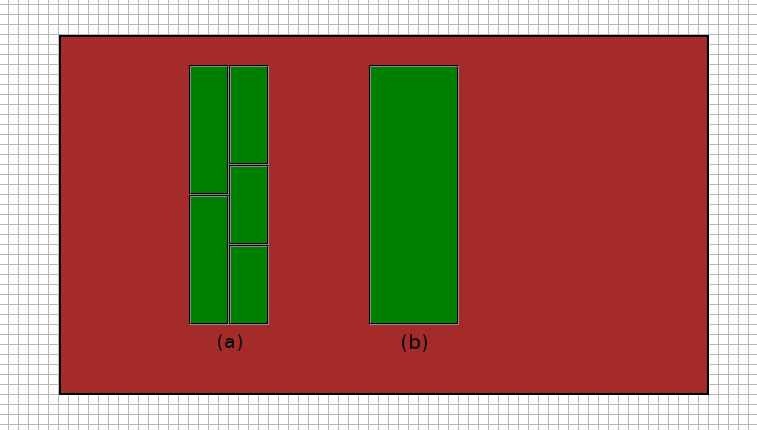
\includegraphics[width=0.80\textwidth]{./imgs/estantes.png}\\[1cm]   
	\caption{A figura (a) mostra uma estante física dividida em várias estantes do Library Mapper enquanto a figura (b)
	mostra apenas uma única estante.}
	\label{variasEstantes}
\end{figure}

 	Essa interpreteção é importante porque dado que o mapa é definido numa superfície 2D não existe outra maneira de separar grupos diferentes de livros numa mesma estante, a não ser colocando uns do lado dos outros.
	\end{itemize}
	
	Outro aspecto desses objetos é que eles podem ter seu tamanho e sua posição mudados dentro da área reservada de desenho do mapa, apenas 
	clicando no objeto e arrastando.Essa propiedade se dá graças ao jQuery e seus métodos {\bf draggable e resizable}.Importante também é o
	fato de tudo isso acontecer apenas dentro dessa área reservada para o desenho do mapa, porque senão a tela ficaria completamente desordenada.
	Essa área é a única que permite que objetos sejam {\it dropados} para a criação de um mapa e isso é possível graças ao método {\bf droppable} do jQuery
	também.
	\subsubsection{JavaScript para Nodes e Nodes para o Banco de Dados}
		Uma vez definido os objetos que formarão o mapa da biblioteca, o usuário clica no botão Save para salvar no banco de dados 
	da aplicação.No meio desse processo existe um passo importante, que é a transformação da informação Web para algo compreensível para
	o Library Mapper poder usar.\\

	A maneira de descrever as partes do mapa como objetos foi proposital, dado que cada uma dessas partes é um objeto do JavaScript, como
	mostrado no exemplo abaixo na criação de um objeto do tipo Shelf.
      \begin{lstlisting}	
	mapObject = new Object();
	var tempType = $(".shelf").eq(i).attr("class").split(' ');
	mapObject.type = tempType[0]; 
	mapObject.id = $(".shelf").eq(i).attr("id");
	mapObject.top = $(".shelf").eq(i).position().top;
	mapObject.left = $(".shelf").eq(i).position().left;
	mapObject.height = $(".shelf").eq(i).height();
	mapObject.width = $(".shelf").eq(i).width();
	mapObject.shelfId = IdEstantes[shelf]; 
      \end{lstlisting}					

	Nesse caso em particular, existe um atributo a mais que é o shelfId, pois o tipo estante é o único com identificador físico.Cada objeto
	obtem suas informações das classes definidas nos botões HTML (bloco, forbidden, qrCode e shelf), que ao serem arrastados geram
	um clone com suas propiedades as quais serão atribuídas a um objeto no momento que o botão Save for clicado.\\

	Esse objeto será adicionado numa pilha junto com todos os que foram criados e, uma vez terminado o empilhamento, a biblioteca JSON se encarrega
	de transformar toda a pilha numa grande String, a qual será passada para o Managed Bean MapBean através de um hidden input do HTML.\\

	Uma vez que essa String é pega pelo MapBean, ele parseia cada item com o auxílio do JSON e transforma em objetos JsonMap, montando um 
	array com cada objeto criado.Após criar esse array de objetos JsonMap ele os divide de acordo com seus tipos em diferentes listas de Nodes,
	ou seja, o tipo bloco vai para uma lista de Node com contentType Free, shelf para uma lista de Node com contentType Shelf, qrCode uma lista 
	de Node com contentType	QrCode e forbidden uma lista de Node com contentType Forbidden.Essa divisão é necessária devida a particularidade de alguns tipos.\\ 

	Durante o processo de transformação toda a área reservada da interface web é ajustada para o padrão do Library Mapper 
	e é montada uma matriz de Nodes.Um exemplo é número de posições que serão ocupadas por uma estante na matriz de Nodes, que é baseado no seu comprimento 
	e largura na interface Web.Essa matriz é mandada para o banco de dados que 
	grava cada nó numa tabela Node, verificando o tipo de cada um para poder também gravar nas tabelas BookShelf e QrCodeMark os respectivos
	tipos Shelf e QrCode desse Node. \\
	
   \subsection{Library Mapper, o usuário}
	Essa seção é reservada para explicar toda a parte relacionada ao usuário da aplicação, que para essa versão do Library Mapper são os visitantes de uma biblioteca.
		
	\subsubsection{Identificando o usuário}
		O primeiro contato que o visitante tem com o Library Mapper é através de um QrCode com o endereço da aplicação e, para
	acessá-lo ele precisa estar perto desse Qr-Code para poder identificá-lo.Portanto, o uso da posição desse Qr-Code parece bastante
	razoável como ponto de partida para a busca do livro que o usuário procura.\\

		A URL contida no Qr-Code possui o endereço para a aplicação com o id desse Qr-Code. A página extrai esse id e manda para o 
	Managed Bean SearchBean.java junto da consulta que o usuário digitar.Esse id é a cordenada XY do QR-Code 
	que o SearchBean guarda durante toda essa seção de busca.Quando esse id é gerado, ele multiplica a posição X do objeto 
	JavaScript por 10 elevado ao número de casas máximo de Y e soma o valor de Y ao resultado.Logo, para obter o inverso é so dividir
	pela mesma potência de 10, atribuindo esse resultado para X e o resto para Y.No exemplo da figura \ref{url},o qual refere-se
	ao Qr-Code da bilbioteca do IME, o número de casas máximo foi 2 pois o maior valor da posição Y é 57.\\
	
	

		\begin{figure}[H]
	\centering
	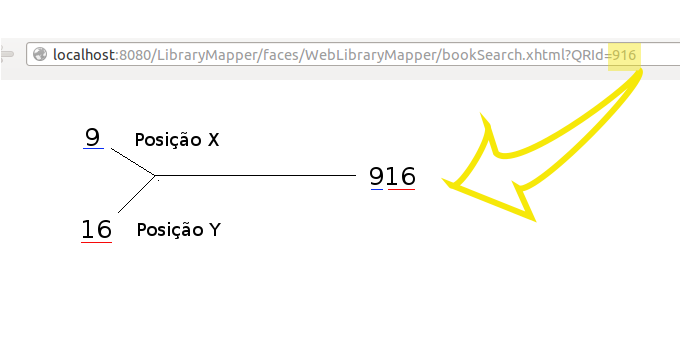
\includegraphics[width=0.50\textwidth]{./imgs/url.png}\\[1cm]   
	\caption{Exemplo de id do Qr-Code passado pela URL}
	\label{url}
\end{figure}
	
	\subsubsection{A consulta e a ligação com a biblioteca}

	Como descrito na seção anterior, o Qr-Code selecionado pelo visitante possui um id com a posição dele no mapa do Library Mapper 
	e uma
	URL para uma página de busca de livros da biblioteca.Nessa página o visitante deve escrever um nome de um livro, ou o autor, 
	ou editora,
	 algo que torne possível reconhecer o livro desejado, para que uma consulta possa ser realizada no banco de dados dessa biblioteca.\\
	
	A consulta é enviada para o SearchBean que chama a classe ServiceWeb.java para montar e enviar a requisição ao serviço da biblioteca.\\

	Como essa busca será realizada no banco de dados da biblioteca, o Library Mapper se restringe a apenas enviar uma consulta para um serviço 
	 dessa biblioteca e esperar por uma resposta desse serviço, pois dessa maneira nenhuma quebra de protocolo de segurança ou ameaça de
	 alteração de 
	dados poderá ser feita.No caso da biblioteca do IME o serviço chamado pertence ao Colméia, onde a consulta é enviada através 
	de uma requisição
	POST e é retornado um XML contendo uma lista de possíveis livros, como mostrado na figura \ref{colmeia}.

		\begin{figure}[H]
	\centering
	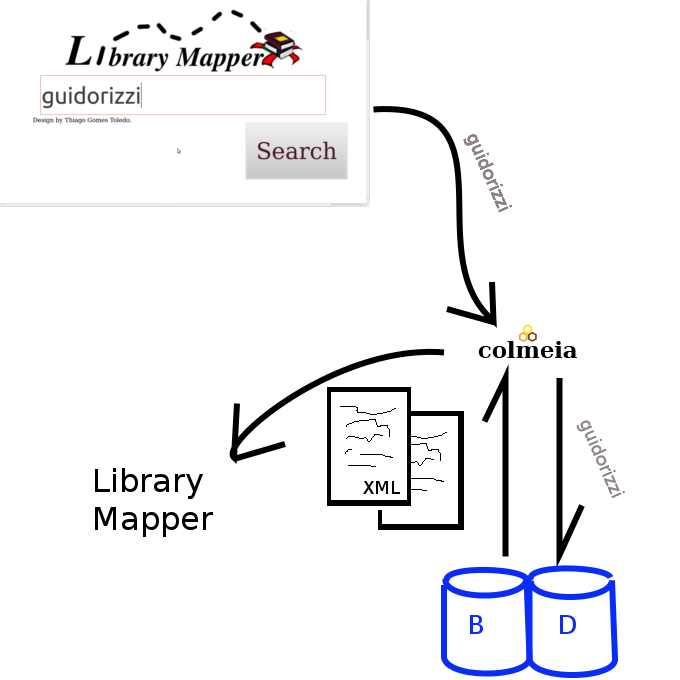
\includegraphics[width=0.45\textwidth]{./imgs/colmeia.png}\\[0.5cm]    
	\caption{Conversa entre Colméia e Library Mapper}
	\label{colmeia}
\end{figure}
	\subsubsection{Lista de livros }
		A lista retornada pelo serviço da biblioteca deve ser {\it tratada}  para que o Library Mapper possa mostrar	 uma lista
	 compreensível para o usuário.
	Como o Colméia retorna um arquivo XML, esse arquivo é parseado com o objetivo de retirar cada livro dessa lista.\\

	Ao receber a lista como resposta ao POST realizado pelo ServiceWeb, o SearchBean envia essa lista para 
	a classe ParseColmeiaXML.java poder
	transformar todo o conteúdo parseado do XML em uma lista de Objetos Books.Caso outra biblioteca não retorne como resposta um XML, 
	 basta criar uma classe no mesmo esquema da ParseColmeiaXML.java, sendo que esta compreenda a resposta enviada
	pelo serviço da biblioteca e fazer o SearchBean chamá-la.\\

	Com os objetos books colocados numa lista, o SearchBean guarda essa lista para ser usada na próxima página que aparecerá
	para o usuário, a bookSelection.xhtml.Nessa página aparecerá essa lista de Books com apenas os títulos de cada livro e um botão 
	Back,
	para realizar uma nova busca, como mostrado na figura.\ref{selectBook} a.

		\begin{figure}[H]
	\centering
	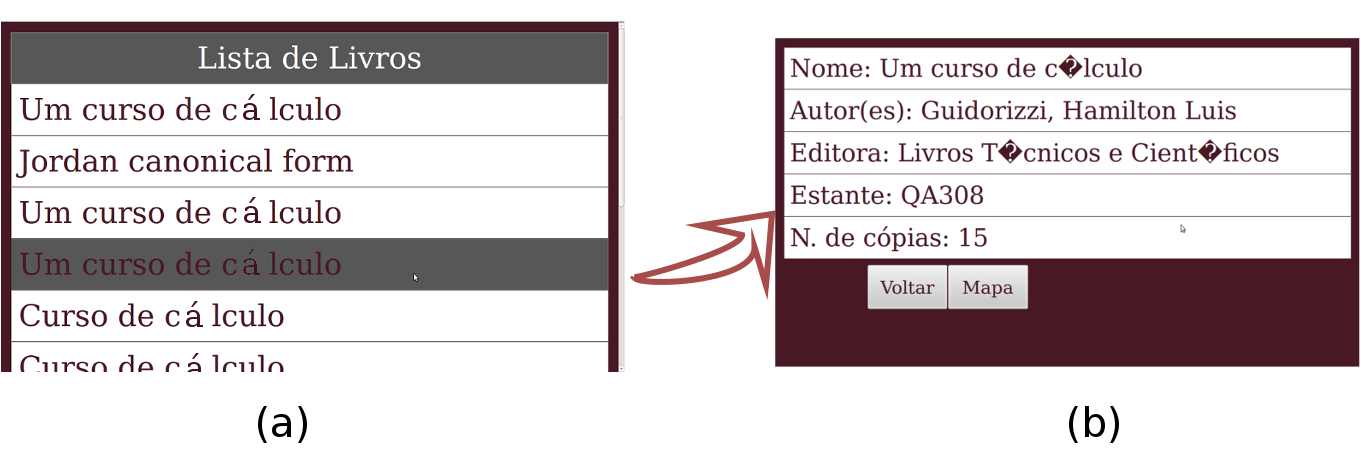
\includegraphics[width=0.75\textwidth]{./imgs/selectBook.png}\\[0.5cm]    
	\caption{Exemplo da lista de livros e a página de informações mostradas para o visitante  }
	\label{selectBook}

\end{figure}
	Quando um livro é selecionado, uma nova página com informações sobre o livro aparecerá o qual será guardado pelo SearchBean (figura.\ref{selectBook} b), para caso o
	usuário realmente queira traçar a rota até esse livro.\\
	
			
	\subsubsection{Montando o mapa com HTML5 e canvas}

	Quando o usuário escolhe traçar o mapa até o livro, o SearchBean cria uma nova instância da classe CanvasMap.java que irá gerar
	o mapa com a rota até o livro em duas etapas:

\begin{itemize}	
	\item{ Desenhando todo o Mapa sem o resultado da busca}

	\item{ Desenhando o resultado da busca por cima do mapa}\\	
\end{itemize}
	Cada Node da matriz da biblioteca é interpretada pelo CanvasMap como um quadrado que varia de cor de acordo com seu ContentType.
	Essa interpretação é feita pelo método {\it createJavaScriptForImpression}, que cria blocos de códigos script CANVAS.
	O CanvasMap irá gerar muitos blocos de linhas de código script CANVAS numa StringBuilder que será escrita no arquivo .xhtml referente 
	ao mapa final do usuário,pois cada um dos Nodes será um bloco a ser transformado.Abaixo segue um exemplo do bloco de um Node com o 
	contentType Forbidden.\\
      \begin{lstlisting}	
	ctx.beginPath();
		ctx.fillStyle = "black";
		ctx.fillRect(0,0,10,10);
	ctx.closePath();
      \end{lstlisting}					

	No GlobalUtils é definido qual o tamanho que cada quadrado deve ter no mapa e as cores escolhidas para esse mapa foram :

\begin{itemize}	
	\item{ Free = white}
	\item{ Forbidden e Shelf(não escolhida)= black}
	\item{ QrCode = yellow }
	\item{ Shelf(escolhida) = blue}
	\item{ Caminho retornado pela busca = red}
\end{itemize}
	Como o script do CANVAS desenhado é lido de cima para baixo, foi mais conveniente sobreescrever antigos blocos criados do que
	verificar se a posição onde esse novo bloco iria ser desenhado já existia para ser editado e por isso, o desenho do mapa é dividido em duas partes, onde a
	primeira desenha todo o mapa e a segunda apenas sobreescreve os blocos existentes com os da rota de busca.\\	  
	
	Quando a primeira busca do Library Mapper é realizada, todo o mapa é buscado do banco de dados, guardado numa matriz no GlobalUtils e 
	só então é gerado o script CANVAS da matriz de Nodes do GlobalUtils.Todo esse processo toma muito tempo, pois carregar todos os dados do
	Banco de dados é uma operação demorada.Contudo a partir dessa busca, todo o mapa desenhado é baseado na matriz que se encontra
	no GlobalUtils, tornando a criação do mapa .xhtml muito mais rápida. 
	\subsubsection{A busca pela estante}

	O CanvasMap recebe do SearchBean três parametros: A StringBuilder que será escrita no arquivo .xhtml, o livro selecionado e o própio SearchBean.
	Após esse passo, o CanvasMap cria blocos script CANVAS para as estantes do livro escolhido e os grava na StringBuilder, para
	finalmente chamar a classe MonitorSearch.java responsável por cuidar da busca.\\

	O MonitorSearch criará duas Threads SearchGrid.java que realizarão a busca bi-direcional, sendo que uma busca sairá da posição da estante
	do livro e outra da do Qr-Code.As buscas feitas por essas duas Threads só pararão quando a flag {\it stopAllOtherTasks} do
	 monitorSearch for setada.\\

	Cada Thread SearchGrid fará uma busca em largura com algumas condições a mais.Da mesma maneira que na BFS clássica, os
	nós do grafo( o grafo nesse caso é a matriz de Nodes) mudam de cor conforme vão sendo visitados e são representados pelo atributo
	{\it color} da classe Node, seguindo o padrão de cores estabelecida no 	\cite{bidirecional}.\\

	Como agora um nó do grafo pode ser alterado por Threads diferentes, podem ocorrer casos das duas Threads estarem vendo o mesmo nó
	ao mesmo tempo.Para isso, cada nó Node possui um semáforo  {\it semaphore} e uma flag {\it estaEmUsoParalelo} que cuidam dessa situação,
	impedindo deadlocks e garantindo exclusão mútua.\\

	Para determinar o final da busca, cada Thread tem três opções:

	\begin{itemize}	
		\item{ A Thread A encontrou o nó destino e a Thread B não chegou a executar.}
		\item{ A Thread A encontrou um nó preto que foi marcado pela Thread B }
		\item{ A Thread A encontrou um nó cinza que foi marcado pela Thread B }\\

			Devido ao segundo e do terceiro caso, durante a busca foi necessário identificar quem tinha marcado cada nó e 
	por isso atribuiu-se a cada Node a variável {\it whoMarkedThisNode}.

	
	\end{itemize}
	
	Caso uma das três situações for atingida,a flag {\it stopAllOtherTasks} é setada e é desenhado o mapa do ponto de encontro
	 das duas Threads até os pontos de origem
	 de cada Thread de busca(Qr-Code
	e estante). Isso só é possível porque cada Node possui dois atributos, parentFromBeginNode e parentFromEndNode que definem os parents de cada
	nó vindo da Thread do início ou do fim da busca.A não ser no caso do nó de encontro, nunca ambos valores estaráo preenchidos e 
	portanto é possível montar a primeira metade, depois a segunda metade e por fim juntar ambas formando o caminho completo.\\

	Esse caminho é uma lista de Nodes que é retornada para o CanvasMap ,o qual se encarrega de criar blocos script CANVAS para desenhar 
	a rota do Qr-Code até a estante onde se encontra o livro.


   \subsection{Caso de Uso}
	O caso de uso para o Library Mapper foi a biblioteca do Instituto de Matemática e Estatística em parceria com
	o sistema de banco de dados Colméia.Foi realizada uma catalogação de
	cada estante e desenhada em proporção todos os itens incluindo estantes, colunas e qualquer obstáculo do primeiro andar dessa biblioteca.
	
	
   \subsection{Resultados e produtos obtidos}
	Com o programa finalizado todas as buscas realizadas por livros do primeiro andar, retornaram com sucesso o caminho certo.Com exceção
	da primeira busca realizada pelo Library Mapper, foi possível encontrar o livro buscado em menos de 2 minutos.
	
   \subsection{Conclusões}
	
	Infelizmente ele não resolve por completo o problema de uma busca por um livro numa biblioteca, pois ainda existe uma grande parcela desse problema atrelado
	a má organização feita pela biblioteca.Contudo como esse é um problema enfrentado por qualquer sistema de busca em ambientes internos, o Library
	Mapper por não apenas encontrar o livro, mas também mostrar o caminho de onde está o visitante até o item que procura é uma ferramenta poderosa e muito eficiente.\\	
	
	O Library Mapper cumpre com excelência o mapeamento de um ambiente interno e auxilía  o visitante desse lugar a encontrar o que 
	procura,levando esse direto ao livro que busca sem perda de tempo ou pasciência, tornando a visita muito mais agradável e proveitosa.
	
   	\newpage
  \section{Parte Subjetiva}
  \subsection{Desafios e frustrações}
	A inexperiência com alguma ferramentas do projeto me tomaram muito tempo durante esse projeto.Em particular:
	\begin{itemize}	
		\item{ 	o jQuery com o métodos droppable, draggable e resizable que foram muito difíceis de configurar e acertar os css
	corretos; }
		\item{ o timeout do Apache-Tomcat.Para montar uma biblioteca como a do IME, levava-se cerca de uma hora e meia para completar tudo
	e nesse tempo a seção expirava.Mas colocando no web.xml do projeto 
\begin{lstlisting}	
    <session-config>  
      <session-timeout>QUANTIDADE EM MINUTOS DE CADA SECAO </session-timeout>  
    </session-config>   
\end{lstlisting}	o problema foi resolvido.Contudo, isso só pode ser setado durante a criação do Mapa.}
		\item{ o synchronized do JAVA não estava funcionando para minha busca paralela e tive que montar meu própio esquema de paralelismo.}\\
	\end{itemize}	

	Um problema frustante foi a maneira como a biblioteca cataloga alguma das suas estantes. Em alguns casos existiam mais de 15 conjuntos
	de livros diferentes, tornando quase impossível nomear uma estante. A solução foram criar várias exceções tratando esses casos, o que 
	aumentou a distância para um modelo mais geral de classificação de estantes numa biblioteca.

	Mas o maior desafio foi desenvolver o projeto nos últimos seis meses em meio a casamento, pintura do apartamento (o qual eu praticamente
	fiz sozinho e foram 2 mãos e em algumas até 3!!), procura de coisas para a casa nova, trabalho de 40 horas semanais, outra matéria da faculdade,
	médico para esposa e arrumação da casa, pois a esposa estava grávida e ainda trabalhando.Esse problema eu ainda não sei bem como foi resolvido,
	mas tomaram algumas madrugadas e todos finais de semana.\\
  \subsection{Relações entre Disciplinas}
\begin{itemize}	
	\item{\bf{Introdução à Computação}}\\

	{\it Eu posso até não saber essa linguagem de programação, mas me dê o manual dela que em uma semana eu te ensino como ela funciona.}\\
	
	Essa foi a frase que eu ouvi no meu primeiro dia no IME pelo professor Roberto Hirata e desde então é dessa maneira que
	tento conduzir minha profissão,aceitando cada desafio que possa me fazer crescer.\\

	Introdução a Computação foi a matéria mais importante que tive no IME, porque foi o primeiro passo para um mundo sem limites, foi onde
	aprendi uma nova linguagem chamada programação, onde eu era capaz de criar tudo que minha imaginação me permitissee por enquanto
	ela me permitiu o Library Mapper.	

	
	\item{\bf{Princípios de Desenvolvimento de Algoritmos}}\\

	Além de aprender conceitos essenciais para desenvolver qualquer programa, como listas ligadas, vetores, pilhas, filas,alguns algoritmos
	de busca (BFS por exemplo) e foi
	onde aprendi com o Professor Arnaldo Mandel que o conhecimento de verdade só chega para aqueles que estudam muito.
	
	
	\item{\bf{Laboratório de programação I e II}}\\

	Em ambas as matérias foi onde comecei a aprender a desenvolver um projeto grande e como dividir esse projeto em pedaços para
	que ele se torne passível de ser resolvido.Mas foi em Laborátorio de programação II onde conheci o conceito do QR-Code e foi onde trabalhei 
	pela primeira vez com essa técnologia.

	\item{\bf{Estrutura de Dados}}\\
		Em estrutura de dados além de aprender novas estruturas de listas ligadas, árvores e buscas referentes a essas estruturas,
	reaforcei muitos conceitos que tinha aprendido anteriormente em Princípios de Desenvolvimento de Algoritmos.
			
	\item{\bf{Algoritmos em Grafos}}\\

	Foi onde aprendi o que é um grafo, toda a parte de busca que pode ser feita nele e quais são os melhores algoritmos de busca
	para cada tipo de grafo.

	\item{\bf{Análise de Algoritmos}}\\
	
	Em análise aprendi de como analisar de verdade um algoritmo e sua complexidade e o quão importante é fazer esse estudo, 
	antes de projetar um software.

	\item{\bf{Conceitos de Programação}}\\

	Foi em conceitos que vi pela primeira vez o conceito de Orientação a Objetos, paradigma usado no Library Mapper.

	\item{\bf{Banco de Dados}}\\
	
	
	\item{\bf{Programação Concorrente, Paralela e Distribuída}}\\
	\item{\bf{XP - eXtreme Programing}} \\
	\item{\bf{Física I e II}}  	\\
\end{itemize}	
  \subsection{Os próximos passos}
  
\bibliographystyle{plain}   
\bibliography{refer}  
\end{document}


